\chapter{Analiza porównawcza}
Naturalnym jest, że frameworki webowe różnią się od siebie pod wieloma względami. Różnice można zauważać od samego początku, czyli idei powstania, poprzez podejście do programisty, na sposobie działania i wydajności kończac. Zwykle przyczyną różnorodności jest sama filozofia frameworka, dążenie do doskonałości. Nie jest możliwe osiągnięcie optymalnych wartości w każdej z dziedzin, które frameworki obejmują, przez co twórcy muszą iść na większe bądź mniejsze kompromisy. Niekiedy owe różnice nie pojawiają się z przymusu, ale z przyjęcia konkretnych założeń.

Są jednak sytuacje, kiedy frameworki są do siebie bardzo podobne. Zwykle są to sytuacje, kiedy framework z jednego języka programowania przenoszony jest do innego języka. Tak było w przypadku opisywanego \textit{Express'a}, który powstał jako odzwierciedlenie frameworka \textit{Sinatra}. Innym przypadkiem występowania podobieństw jest chęć wykorzystania jakiegoś fragmentu frameworka, który uznawany jest za standard i bez którego programista musi posiadać większą wiedzę aby odpowiednio wykorzystywać framework.\\

W kolejnych podrozdziałach zostaną przedstawione porównania wybranych frameworków na zasadzie \textit{,,każdy z każdym''}. Poza podobieństwami i różnicami w budowie oraz idei działania, zamieszczona została subiektywna opinia autora na temat sytuacji, w których jeden framework ma przewagę nad drugim.

\section{Ruby on Rails vs Phoenix}
Jako pierwsze analizie porównawczej zostaną poddane najstarszy i najmłodszy framework spośród opisywanych, czyli \textit{Ruby on Rails} oraz \textit{Phoenix}. Owa różnica ,,wieku'' mocno rzutuje na całokształ tych frameworków.  Pierwszy ma już stabilną, wręcz nienaruszalną, pozyję na rynku, bardzo dużą społeczność oraz niezliczoną ilość materiałów dostępnych w Internecie.
Drugi natomiast, co oczywiście jest efektem wielu składowych, ma spory potencjał. Oczywiście nie jest to pierwszy, ani jedyny, framework, który owy potencjał posiada. Jednakże w przypadku \textit{Phoenix'a} jest duża szansa, iż będzie on wykorzystany. Przyczynić się do tego może środowisko programistów \textit{Ruby on Rails}, ponieważ już teraz duża ilość programistów albo mocno się \textit{Phoenixem} interesuje, albo zdecydowało się zmienić technologię na \textit{Elixir'a} i \textit{Phoenix'a}.

% !!filozofia działania
% idea powstania
% !!architektura, elementy składowe
% !!wygoda użytkowania
% szybkość powstawania aplikacji
% !!dostępność najczęściej wykorzystywanych bibliotek (system użytkowników, zapisywanie plików w chmurze, przetwarzanie w tle)
% testowanie aplikacji

\subsection{Filozofia działania}
\textit{Ruby on Rails} oraz \textit{Phoenix} posiadają elementy wspólne jeśli chodzi o sposób działania. Jest to spowodowane faktem, iż z założenia \textit{Phoenix} miał wykorzystywać najlepsze elementy z innych frameworków.

Jeśli chodzi o filozofię działania, oba frameworki są zgodne w kwestii chęci ułatwienia pracy programistom. Zarówno \textit{Ruby on Rails}, jak i \textit{Phoenix}, mocno uwypuklają przyjemność korzystania z języków programowania, na których są oparte. Twórcy \textit{Ruby on Rails} zapoczątkowali trend stawiania na przyjemność użytkowania w świecie frameworków webowych, natomiast twórcy \textit{Phoenix} bardzo dobrze to zaimplementowali w swoim frameworku. Z tego też powodu spora część programistów \textit{Ruby on Rails} interesuje się rozwojem \textit{Phoenix'a}.\\

Podstawową różnicą w filozofii działania jest kwestia szybkości działania. Twórca \textit{Ruby on Rails} nie poświęcił ani jednego punktu w \emph{,,The Ruby on Rails Doctrine''} \cite{rails_doctrine}. Można z tego faktu wyciągnąć wniosek, że szybkość działania \textbf{nie jest} kluczowa dla tego frameworka. I powszechna opinia na temat \textit{Rails'ów} to potwierdzi. Nie zmienia to jednak faktu, że wiele bardzo dużych portali opartych jest na \textit{Ruby on Rails}. Przykładami mogą być \textit{GitHub}, \textit{Groupon}, \textit{AirBnB} czy \textit{Kickstarter}. Framework ten jest natomiast idealnym narzędziem do szybkiego tworzenia aplikacji. \textit{Ruby on Rails} na pewno zyskało wielu użytkowników ze względu na szybkość prototypowania, co jest bardzo istotne w dobie \textit{start-up'ów}.

Dla odmiany, \textit{Phoenix} szczyci się swoją wysoką wydajnością. Jest to jeden z filarów tego frameworka. Co ciekawe, pomimo postawienia na szybkość działania, nie ucierpiała na tym szybkość prototypowania. Powodów takiego stanu rzeczy po raz kolejny można doszukiwać się w języku programowania, na którym oparty jest \textit{Phoenix}. Tworzy to sporą przewagę nad \textit{Ruby on Rails} w przypadkach, gdzie poza szybkością powstania aplikacji równie ważna jest jej wydajność.

\subsection{Architektura aplikacji, elementy składowe}
Zarówno \textit{Ruby on Rails}, jak i \textit{Phoenix} są frameworkami typu full-stack. Oznacza to, że dostarczane są z mechanizmami odpowiedzialnymi za:
\begin{itemize}
  \item serwer http - przy pomocy którego można uruchomić aplikację w środowisku developerskim,
  \item generowanie struktury projektu (architektura MVC),
  \item połączenie z bazą danych - adaptery do różnych typów baz danych, ORM,
  \item router aplikacji - odpowiedzialny za przekierowywanie zapytań do odpowiednich akcji kontrolerów,
  \item podstawowe mechanizmy bezpieczeństwa (mechanizm sesji, bezpieczne ciasteczka),
  \item silniki szablonów - Slim, HAML,
  \item wysyłanie wiadomości e-mail z aplikacji - należy jedynie skonfigurować serwer SMTP z którego ma korzystać aplikacja.
\end{itemize}

Wykorzystywana w obu frameworkach architektura została pokazana na rysunku \ref{fig:rails_architecture}.
\newpage
% http://www.sentex.net/~pkomisar/Ruby/Rails2.png (?)
\begin{figure}[h]
  \centering
  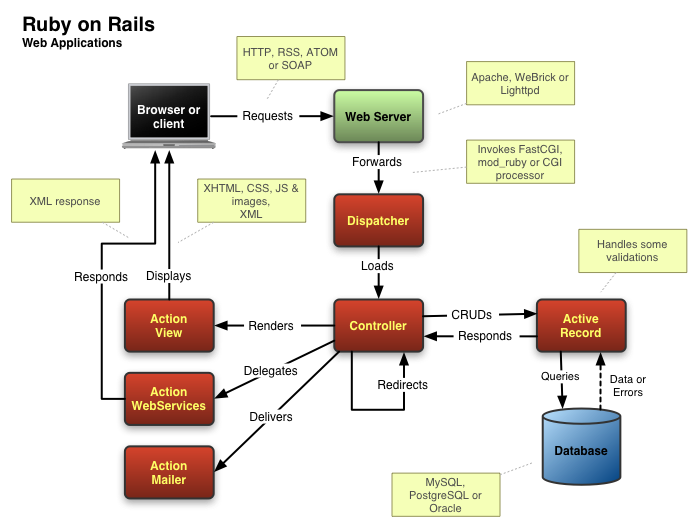
\includegraphics[width=\linewidth]{images/rails_architecture}
  \caption{Architektura Ruby on Rails.\\Źródło: \url{http://www.sentex.net/~pkomisar/Ruby/Rails2.png}}
  \label{fig:rails_architecture}
\end{figure}

\subsection{Wygoda użytkowania, szybkość powstawania aplikacji}
W kwestii wygody użytkowania oba frameworki są na podobnym poziomie. Zarówno \textit{Ruby on Rails} jak i \textit{Phoenix} są stworzone w taki sposób, aby ułatwić prototypowanie aplikacji. Dzięki temu odczucia z użytkowania obu są bardzo przyjemne. Aplikacje można tworzyć relatywnie szybko, frameworki posiadają praktycznie wszystkie niezbędne mechanizmy, które wykorzystywane są w większości aplikacji webowych.

Przykładowe mechanizmy, które były brane pod uwagę:
\begin{itemize}
  \item przetwarzanie danych w tle - w przypadku \textit{Ruby on Rails} jest to \textit{Sidekiq}, jego odpowiednikiem w \textit{Phoenix'ie} jest \textit{Akira},
  \item autentykacja/autoryzacja użytkowników, zarządzanie sesją - \textit{Devise} dla \textit{RoR} oraz \textit{Addict} dla \textit{Phoenix'a},
  \item wsparcie dla dołączania skryptów JavaScript w warstwie prezentacji,
  \item wsparcie dla różnych preprocesorów styli (Sass, Less)
\end{itemize}

Istnieje jednak pewna różnica, która może mieć wpływ na wygodę programisty, a jest nim rodzaj języka programowania. Dużo bardziej popularne jest podejście obiektowe, na którym oparty jest \textit{Ruby}. \textit{Elixir} natomiast jest językiem funkcyjnym. Paradygmat funkcyjny różni się znacznie od obiektowego, przez co w przypadku braku znajomości tego paradygmatu, używanie \textit{Phoenix'a} może być dużo trudniejsze. Zasada ta działa oczywiście w dwie strony i jeśli ktoś nie zna podejścia obiektowego, korzystanie z \textit{Ruby on Rails} również może być utrudnione.

\subsection{Podsumowanie}
Oba frameworki są do siebie podobne w kwestii używania. Bardzo ciekawe oraz pomocne są materiały, które wyjaśniają dlaczego dany framework powstał oraz jak powinien być używany, aby w pełni wykorzystać jego potencjał. Przewagą \textit{Ruby on Rails} jest na pewno dojrzałość oraz ogromna społeczność. W kwestii, oczywiście subiektywnej, przyjemności z korzystania, oba frameworki są na podobnym poziomie. \textit{Phoenix} zyskuje przewagę w kwestii wydajności. Moim zdaniem w tym frameworku drzemie niesamowity potencjał i mam nadzieję, że na stałe wpisze się w zbiór najbardziej popularnych frameworków webowych.

\section{Ruby on Rails vs Express}
Zestawienie \textit{Ruby on Rails} oraz \textit{Express'a} jest zestawieniem najstarszych frameworków spośród narzędzi wybranych do analizy. Pierwszy powstał w 2004 roku, drugi natomiast swój początek miał w 2010r. Ze względu na swój wiek oba frameworki mają ugruntowaną pozycję na rynku oraz rzesze użytkowników.

\subsection{Filozofia działania}
W przypadku zestawienia \textit{Ruby on Rails} oraz \textit{Express'a} filozofia działania oraz sama idea powstania są kluczowymi aspektami. Wynika to z faktu, iż \textit{Express} powstał z chęci przeniesienia frameworka \textit{Sinatra} z środowiska programistów Rubiego do środowiska \textit{Node.js}. Framework \textit{Sinatra} powstał natomiast jako kontra do rozbudowanego \textit{Ruby on Rails}. Z tego też powodu \textit{Ruby on Rails} oraz \textit{Express.js} są swoimi przeciwnościami.

Z jednej strony mamy framework typu full-stack i podejście \textit{Convention over Configuration}. Z drugiej - minimalistyczny framework, do którego możemy (ale nie musimy) dołączyć szereg bibliotek, żeby w kwestii funkcjonalności zrównać się z \textit{Ruby on Rails} oraz oczywiście podejście \textit{Configuration over Convention}. Przejście z jednego świata do drugiego bywa dość nieprzyjemne, wymaga dużej czujności programisty oraz większych nakładów pracy. Dlatego też środowiska programistów \textit{Ruby on Rails} oraz \textit{Express'a} rzadko kiedy się przenikają.

Ze względu na ideę powstania każdego z nich, trudno wskazać elementy łączące \textit{Ruby on Rails} oraz \textit{Express'a}. Oba służą do tworzenia aplikacji internetowych, robią to jednak w różny sposób.

\subsection{Architektura aplikacji, elementy składowe}
\label{rails_express:architektura}
Różnice w kwestii architektury aplikacji oraz bibliotek, które się składają na framework, są w przypadku \textit{Ruby on Rails} oraz \textit{Express'a} bardzo łatwe do zauważenia. Wynika to ze złożoności samych frameworków, a więc podejścia typu \textit{full-stack} w przypadku \textit{Ruby on Rails} oraz minimalizmu \textit{Express'a}. Pierwszy posiada praktycznie wszystko, co jest wymagane do stworzenia podstawowej aplikacji internetowej. W przypadku \textit{Express'a} niestety wymagany jest dodatkowy wysiłek programisty w celu stworzenia aplikacji. Podstawowym problemem jest brak dołączonych adapterów umożliwiających połączenie z bazą danych. Framework ten nie posiada również mechanizmu umożliwiające mapowanie obiektowo-relacyjne (ang. \textit{ORM} - Object-Relational Mapping).

Jako, że \textit{Express} nie posiada wbudowanego generatora projektu, projekt nie posiada określonej struktury. Z jednej strony daje to swobodę działania programiście, czego niekiedy brakuje w \textit{Ruby on Rails}. Niewątpliwie możliwość wykorzystania innej architektury aplikacji niż MVC jest mile widzianą cechą. Z drugiej zaś strony może być problematyczne w sytuacji, kiedy każdy projekt ma swoją ,,autorską'' strukturę i nie przestrzega żadnego schematu.

\subsection{Wygoda użytkowania, szybkość powstawania aplikacji}
Porównianie wygody użytkowania oraz szybkości powstawania aplikacji w przypadku \textit{Ruby on Rails} oraz \textit{Express'a} w dużym stopniu odnosi się do sekcji \ref{rails_express:architektura}. Struktura aplikacji oraz biblioteki dołączone do frameworka są kluczowe dla programistów, szczególnie początkujących. W połączeniu z brakiem domyślnych mechanizmów mapowania obiektowo-relacyjnego, można odnieść wrażenie, iż \textit{Express} nie jest najlepszym frameworkiem dla początkujących programistów. Należy dobrze poznać środowisko, żeby móc wybrać dobrze współpracujące ze sobą komponenty i dopiero wtedy można zacząć tworzyć aplikację. Pod tym względem zupełnym przeciwieństwem jest \textit{Ruby on Rails}. Programista nie musi znać całego środowiska oraz dużej ilości bibliotek, żeby stworzyć aplikację. Jednakże w momencie, kiedy zajdzie taka potrzeba, możliwa jest podmiana niektórych bibliotek bądź też rezygnacja z części w celu zmniejszenia rozmiarów projektu.

\subsection{Podsumowanie}
Wrażenia po korzystaniu z obu frameworków są zgoła odmienne. I oczywiście znacząco zależą od wcześniejszych doświadczeń i przyzwyczajeń w kwestii tworzenia aplikacji internetowych. Osoba, która dopiero zaczyna swoją przygodę z tą dziedziną informatyki może mieć pewne problemy aby zacząć pracę z \textit{Express'em}. Jego modułowość oraz lekkość są w stanie wykorzystać i docenić osoby, które posiadają pewne doświadczenie w kwestii aplikacji webowych oraz wiedzą dokładnie jakich komponentów będą musieli użyć w celu stworzenia aplikacji. Frameworkiem dużo bardziej przyjaznym dla początkujących oraz przy tworzeniu standardowych aplikacji jest \textit{Ruby on Rails}. Programista może, ale oczywiście nie musi, skorzystać z dostarczonych przez twórców rozwiązań, które w większości przypadków są wystarczające.

Zdecydowaną zaletą \textit{Express'a} jest popularność języka programowania \textit{JavaScript}. Zdecydowanie zmniejsza to barierę wejścia w środowisko tego frameworka.

\section{Phoenix vs Express}
Ostatnim porównaniem jest konfrontacja \textit{Phoenix'a} z \textit{Express'em}. Z jednej strony mamy bardzo młody framework typu full-stack, z drugiej niewielki, ale sprawdzony framework, który stawia na minimalizm i modularność. Zestawienie to jest o tyle ciekawe, iż \textit{Phoenix} miał wykorzystywać najlepsze elementy innych frameworków, lecz ciężko doszukać się tam rozwiązań znanych z \textit{Express'a}.

\subsection{Filozofia działania}
Podobnie, jak w przypadku zestawienia \textit{Ruby on Rails} z \textit{Express'em}, filozofia powstania znacząco różni się w przypadku \textit{Phoenix'a} i \textit{Express'a}. Pierwszy jest młodym frameworkiem, który wzoruje się na najlepszych rozwiązaniach, oczywiście subiektywnie wybranych przez twórców, z innych frameworków webowych w celu zapewnienia maksymalnego zadowolenia programisty oraz osiągnięcia wysokiej wydajności. Drugi natomiast preferuje dostarczenie jedynie niezbędnych mechanizmów, stawiając na podejście \emph{Configuration over Convention}.

Wyższość jednego podejścia nad drugim jest oczywiście kwestią dyskusyjną. Jednakże porównując liczbę frameworków podobnych do \emph{Phoenix'a}, a więc typu full-stack oraz podobnych do \emph{Express'a}, czyli minimalistycznych, nie trudno zauważyć jak bardzo popularne jest pierwsze podejście.

\subsection{Architektura aplikacji, elementy składowe}
Nietrudno zauważyć, że \emph{Phoenix} ma niewiele wspólnego z \emph{Express'em} w kwestii architektury aplikacji. Sam fakt, iż \emph{Phoenix} jest frameworkiem typu full-stack, definiuje podstawową różnicę. Ponownie, problemem jest tutaj przede wszystkim brak adaptera do baz danych oraz mechanizmu ORM w wypadku \emph{Express'a}. Jest to na tyle często wykorzystywana funkcjonalność, że framework do tworzenia aplikacji działających po stronie serwera powinien mieć wbudowane takie mechanizmy. \emph{Phoenix} narzuca programiście model \emph{MVC}, gdzie \emph{Express} daje dowolność w kwestii użytego wzorca architektonicznego. Jest to z pewnością zaletą \emph{Express'a}, ponieważ model \emph{MVC} jest najbardziej uniwersalny, jednak są sytuacje gdzie inne podejścia dużo lepiej się sprawdzają.

\subsection{Wygoda użytkowania, szybkość powstawania aplikacji}
\emph{Phoenix} jest frameworkiem bardziej uniwersalnym. Można przy jego pomocy bardzo szybko stworzyć aplikację internetową, która korzysta z bazy danych i innych prostych mechanizmów, np. posiada autentykację użytkowników. Wbudowane mechanizmy pozwalają na realizację takiej funkcjonalności w bardzo szybkim czasie i bez dużych nakładów pracy. Problemem w przypadku \emph{Phoenixa} może być paradygmat funkcyjny języka \emph{Elixir}. Aby poprawnie pisać aplikacje z wykorzystaniem tego języka należy poznać programowanie funkcyjne, które jest dużo mniej popularne niż programowanie obiektowe.

\emph{Express}, przynajmniej na początkowym etapie tworzenia aplikacji wymaga od programisty znajomości środowiska oraz bibliotek, które w innych frameworkach uznawane są jako podstawowe. Do momentu, aż programista posiada wyrobione zdanie na temat dostępnych bibliotek, korzystanie z \emph{Express'a} nie jest tak szybkie, jak z \emph{Phoenix'a}.

\subsection{Podsumowanie}
Nie da się ukryć, że porównywane frameworki stoją poniekąd po dwóch stronach barykady. Jest to konfrontacja kompletnego frameworka typu full-stack z frameworkiem, który powstał jako zaprzeczenie tej idei. Oba rozwiązania mają oczywiście swoich fanów oraz przeciwników. Nie da się jednoznacznie wyłonić lepszego z tych dwóch rozwiązań, ponieważ ich przydatność w dużym stopniu zależy od rodzaju aplikacji, jaki mamy wykonać oraz znajomości danego środowiska.

Biorąc pod uwagę podejście obu frameworków do tworzenia aplikacji, \emph{Phoenix} stanowczo jest wygodniejszym narzędziem. Framework ten stworzony jest do szybkiego prototypowania i jak najbardziej się sprawdza w takim zastosowaniu. Przeszkodą dla wielu programistów może być natomiast funkcyjny język programowania \emph{Elixir}, na którym oparty jest \emph{Phoenix}.

\emph{Express} natomiast sprawdza się jako narzędzie do stworzenia aplikacji internetowej, która nie jest dużych rozmiarów. Podstawowe elementy tego frameworku, jak router zapytań i system widoków, idealnie się nadają do tego typu zastosowań. Problemy zaczynają się dopiero, kiedy aplikacja musi mieć bezpośrednie połączenie z bazą danych oraz wymagane są dodatkowe, bardziej zaawansowane mechanizmy.
